\chapter{Tabelle hash}

{{[}CLRS{]} pp. 209-211}

{Le tabelle hash sono una possibile implementazione dei dizionari,insiemi dinamici con inserimento, cancellazione e ricerca dove ogni elemento è associato ad una chiave.}

{I dizionari possono essere implementati nei seguenti modi:}

\begin{itemize}
\tightlist
\item
  {Liste: $O(n)$}
\item
	{Alberi binari}

\begin{itemize}
\tightlist
\item
  	{Non bilanciati: $O(n)$}
\item
  	{Bilanciati: $O(log(n))$}
\end{itemize}

\item
  	{Tabelle hash}

\begin{itemize}
\tightlist
\item
	{Tempo medio: $\Theta(1)$ (Motivo principale per l'utilizzo delle tabelle hash)}
\item
	{Caso peggiore: $\Theta(n)$}
\end{itemize}

\end{itemize}

{Vogliamo fornire un'applicazione che ha bisogno di un insieme dinamico (insert/delete/search). Ogni elemento ha una chiave estratta da un universo $\mathbb{U}$ con $\abs{\mathbb{U}} = \{0,\ldots,w-1\}$, dove $w$ non è troppo grande. Nessun elemento ha la stessa chiave (elementi distinti). }

{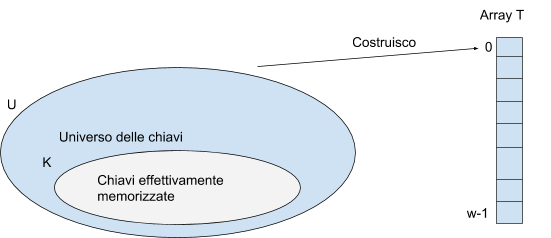
\includegraphics{images/image521.png}}

{Mi costruisco una tabella ad accesso diretto. Si può utilizzare un array $[0,\ldots,w-1]$ dove}

\begin{itemize}
\tightlist
\item
  {ogni posizione (o cella) corrisponde ad una chiave di $\mathbb{U}$}
\item
  {Se c'è un elemento $x$ con chiave $k$, allora nella posizione $T(k)$ è contenuto un puntatore a $x$}
\item
  {Altrimenti, se l'insieme non contiene l'elemento, $T(k) = NULL$}
\end{itemize}

\begin{equation}
T(k) =
\begin{cases}
x & \mbox{se } x.key=k, x\in K \\
NULL & \mbox{altrimenti}
\end{cases}
\end{equation}

{Direct\_Access\_Search : }$O(1)$

\lstinputlisting{code/direct_access_search.txt}

{Direct\_Access\_Insert : $O(1)$}

\lstinputlisting{code/direct_access_insert.txt}

{Direct\_Access\_Delete : $O(1)$}

\lstinputlisting{code/direct_access_delete.txt}

{Potrebbe essere uno spreco se $\abs{K} \ll \abs{\mathbb{U}}$ (Molto minore)}

{Pregi:}

{Operazioni eseguibili in tempo costante}

{Difetti:}

{Lo spazio utilizzato è proporzionale a $w$ e non al numero $n$ di elementi. Di conseguenza si può avere un importante spreco di memoria.}

{Per ovviare al problema dello spreco di memoria si utilizzano le tabelle hash.}

{Richieste:}

\begin{enumerate}
\tightlist
\item
  {Vogliamo ridurre lo spazio per la tabella ad $\Theta(\abs{K})$, ovvero il numero di chiavi
  effettivamente utilizzate}
\item
  {Le operazioni siano con costo medio $\Theta(1)$, ma non nel caso pessimo}
\end{enumerate}

{Idea:}

{Invece di memorizzazione un elemento con chiave o nella cella $k$, si usa una funzione $h$, detta funzione hash, e si memorizza l'elemento nella cella $h(k)$}


{$h:\mathbb{U}\rightarrow\{0,1,\ldots,m-1\}$, dove $m$ della tabella hash è generalmente molto più piccola della dimensione dello spazio di tutte le chiavi.}

{Problema: }

{Se $m < \abs{\mathbb{U}}$, due valori possono essere mappati nella stessa cella, ciò è chiamato collisione. }

{Le tabelle hash possono soffrire del problema delle collisioni: quando un elemento da inserire è mappato, tramite $h$, in una cella già occupata, si verifica una collisione.}

$k_1 \neq k_2 \in \mathbb{U}, h(k_1) = h(k_2)$

{Se $\abs{K} > m$, ho la certezza di imbattermi in collisioni.}

{Cerchiamo quindi strategie per gestire le collisioni, ne analizzeremo due:}

\begin{enumerate}
\tightlist
\item
  {Metodo di concatenamento (liste di collisione (o di trabocco))}
\item
  {Indirizzamento aperto}
\end{enumerate}

\subsection{Risoluzione delle collisioni tramite metodo di concatenamento}

{Si mettono tutti gli elementi che sono associati alla stessa cella in una lista concatenata.}

{La cella $j$ contiene un puntatore alla testa di una lista di tutti gli elementi memorizzati che sono mappati in $j$. Se non ci sono elementi, la cella $j$ conterrà $NULL$.}

\subsubsection{Implementazioni}

{Andiamo ad analizzare l'hashing con concatenamento.}

\lstinputlisting{code/chained_hash_insert.txt}

{Tempo di esecuzione: $\Theta(1)$ se $h$ impiega tempo costante $\Theta(1)$ e l'elemento non è presente nella lista}

\lstinputlisting{code/chained_hash_search.txt}

{Tempo di esecuzione:}

{~~~~~~~~Caso peggiore:}

{~~~~~~~~~~~~~~~~Proporzionale alla lunghezza della lista nella cella $h(x)$}

\lstinputlisting{code/chained_hash_delete.txt}

{Tempo di esecuzione:}

{Caso peggiore:}

{$\Theta(1)$ se la lista doppiamente concatenata (ci serve un puntatore al predecessore)}

{Senza una lista doppiamente concatenata servirebbe ricercare la chiave del predecessore come ulteriore step.}

{Sia T una tabella hash con n celle dove sono stati memorizzati $n$ elementi. }

{Caso peggiore:}

{Tutti gli elementi sono mappati nella stessa cella. Abbiamo quindi
un'unica lista di lunghezza $n$.}

{Tempo di esecuzione della ricerca: $\Theta(n)$}

{Caso medio:}

{Analisi di $h$}

{Deve soddisfare la proprietà di }{Hashing Uniforme Semplice:}

{Ogni elemento ha la stessa probabilità di essere mandato in una qualsiasi delle $m$ celle, indipendentemente dalle celle in cui sono mancati gli altri elementi.}

$\forall i \in \{0,\ldots,n-1\}, Q(i) = \frac{1}{n}$

{Assumo che $h$ soddisfi la proprietà di Hashing Uniforme Semplice: indico con $n_j$ la lunghezza della lista $T[j]$}

{Il valore medio di $n_j$ è $\alpha=\frac{n_0+n_1+\ldots+n_{m-1}}{m}=\frac{n}{m}$}

{Fattore di carico: }

{In una tabella hash con $n$ chiavi ed $m$ celle, il fattore di carico è $\alpha = \frac{n}{m}$. Esso è il numero medio di elementi memorizzati in ogni lista.}

\paragraph{Teorema 1}

{In una tabella hash in cui le collisioni sono risolte con il concatenamento, una ricerca senza successo richiede, nel caso medio, un tempo $\Theta(1+\alpha)$, nell'ipotesi di Hashing Uniforme Semplice.}

{Intuizione:}

\begin{itemize}
\tightlist
\item
  {Calcolo $i=h(k)$: $\Theta(1)$}
\item
  {Accedo a $T[j]$ : $\Theta(1)$}
\item
  {Scorro la lista $T[j]$ fino alla fine) : $\Theta(\alpha)$ (in media)}
\end{itemize}

\paragraph{Teorema 2}

{In una tabella hash in cui le collisioni sono risolte con il concatenamento, una ricerca con successo richiede, nel caso medio,un tempo $\Theta(1+\frac{\alpha}{2}) = \Theta(1+\alpha)$ nell'ipotesi di Hashing Uniforme Semplice.}

{Se il numero di celle della tabella hash è almeno proporzionale al numero di elementi da memorizzare, cioè abbiamo $n=O(m)$, di conseguenza \\ $\alpha=\frac{n}{m} = \frac{O(m)}{m}=\Theta(1)$. (Se alpha è costante) }

Tutte le operazioni quindi, mediamente, sono svolte in tempo $\Theta(1)$.


\subsubsection{Come si costruiscono le funzioni hash?}

{Significato di hash: polpetta, tritare.}

{Una buona funzione hash dovrebbe essere in grado di distribuire in modo
uniforme le chiavi nello spazio degli indici della tabella. Deve quindi
rispettare l'ipotesi di HUS.}

{Esempio: la distribuzione delle chiavi è nota.}

{Le chiavi sono numeri reali $k$ casuali e distribuiti in modo indipendente e uniforme nell'intervallo $0 \leq k \leq 1$.}

{Per distribuirle su $m$ celle possiamo moltiplicarle per il valore di quest'ultimo: $h(k) = \floor{km}$}

{Questa funzione soddisfa l'ipotesi HUS.}

{Le distribuzioni delle chiavi difficilmente risultano note a priori. }

{Metodi di costruzione delle funzioni hash.}

\begin{enumerate}
\tightlist
\item
  {Metodo della divisione}
\end{enumerate}

{}

$h(k) = k\,mod\,m$

{~~~~~~~~Esempio: }

$h=10,\,k=91,\,h(k)=91\,mod\,19=15$

{}

{Svantaggio: }

{Scegliere il valore di m diventa critico. }

{}

{Vantaggio:}

{Semplice da implementare}

{}

{~~~~~~~~Come scegliere m:}

{Si evitano le potenze di due per non ottenere sempre e solo i p bit
meno significativi ed evitare problemi (carattere uguale di fine
stringa). Scegliamo un numero primo non troppo vicino ad una potenza
esatta di 2 o 10.}

{Es: 3 collisioni accettabili, $n=2000,\frac{n}{3}=666$, perciò $m=701$}

\begin{enumerate}
\setcounter{enumi}{1}
\tightlist
\item
  {Metodo della moltiplicazione}
\end{enumerate}

{~~~~~~~~Se $x \in [0\ldots1]$ uniformemente distribuiti}

$h(x) = \floor*{m*x}$

{~~~~~~~~Data una chiave naturale, la trasformo in un numero nell'intervallo $[0\ldots1]$ per poi moltiplicarlo per $m$.}

{~~~~~~~~Fisso una costante $A, 0 \leq A \leq 1$}

{~~~~~~~~Calcolo $K*A$ ed estraggo la parte frazionaria}

\begin{equation}
(K*A)\,mod\,1 = k * A - \floor*{k*A}
\end{equation}

\begin{equation}
h(x) = \floor*{m*(K*A)\,mod\,1}
\end{equation}

{Vantaggio:}

{Il valore di $m$ non è più critico. Funziona bene con tutti i valori di A. Knuth suggerì il valore $\frac{\sqrt{5}-1}{2}$.}


{~~~~~~~~Per semplificare i conti possiamo scegliere $m=2^p$}

{$A = \frac{q}{2w} = $ lunghezza di una parola in memoria, $0<q<2^w$ intero.}

{~~~~~~~~Ipotesi:}

{$k$ entra in una sola parola: $k*a = mod 1 = \frac{k*q}{2^w}\,mod\,1$}

{$h(k)=p$ bit più significativi della parola meno significativa di $k*q$.}

\begin{enumerate}
\setcounter{enumi}{2}
\tightlist
\item
  {Hashing universale}
\end{enumerate}

{Se un avversario conosce la funzione hash, qualunque essa sia, potrebbe inserire nella tabella elementi che finiscono tutti nella stessa cella e ciò porterebbe a pessime prestazioni.}

{La soluzione è costruire un insieme di funzioni hash da pescare casualmente.}

\begin{enumerate}
\tightlist
\item
  {~Costruisco un insieme h di funzioni hash, l'insieme deve essere
  opportunamente costruito.}
\item
  {Il programma sceglie casualmente h dall' insieme}
\end{enumerate}

\subsection{Risoluzione delle collisioni tramite indirizzamento aperto}

{Ipotesi: }

{Non ho alcuna struttura ausiliaria esterna.}

{Idea:}

{Gli elementi sono tutti memorizzati nella tabella.}

{Non c'è memoria esterna}

{Ogni cella contiene un elemento dell'insieme dinamico oppure $NULL$}

{Per cercare un elemento di chiave $k$:}

\begin{enumerate}
\tightlist
\item
  {Calcoliamo $h$ ed esaminiamo la cella con indice (ispezione)}
\item
  {Se la cella contiene la chiave $k$, la ricerca ha successo. }
\item
  {Se invece contiene $NULL$, la ricerca termina senza successo.}
\item
  {Se la cella contiene una chiave che non è $k$ calcoliamo l'indice di un'altra cella in base a $k$ e all'ordine di ispezione. Si continua la scansione della tabella finché non si trova $k$ (successo), una cella contenente $NULL$ oppure dopo $m$ ispezioni senza successo.}
\end{enumerate}

{La funzione hash per l'indirizzamento aperto è la seguente:}

\begin{equation}
h:\mathbb{U}x\{0,0,\ldots,m-1\} \rightarrow \{0,0,\ldots,m-1\}
\end{equation}

{$h(k,i)$ rappresenta la posizione della chiave $k$ dopo $i$ ispezioni fallite}

{per ogni chiave, la sequenza di ispezioni data da \\
$<h(k,0),h(k,1),\ldots,h(k,m-1))>$ deve essere una permutazione di $<0,1,\ldots,m-1>$ \\ in modo che ogni posizione della tabella hash possa essere considerata come possibile cella in cui inserire una nuova chiave.}

{Assunzioni:}

{~~~~~~~~gli elementi della tabella hash sono senza dati satellite}

{Hash insert: restituisce l'indice della cella dove ha memorizzato la chiave $k$, oppure segnala un errore se la tabella è piena}

\lstinputlisting{code/hash_insert.txt}

{Hash search: restituisce $j$ se $T[j]$ contiene la chiave $k$ oppure $NULL$ se essa non esiste in $T$.}

\lstinputlisting{code/hash_search.txt}

{Problema:}

{La cancellazione da una tabella hash con indirizzamento aperto è problematica. }

{Soluzione:}

{Non si può cancellare ponendo $NULL$ al posto della chiave. Usiamo quindi un marcatore (un valore speciale, chiamato ``deleted'') al posto di $NULL$ per marcare una cella come vuota a causa di un'eliminazione.}

{Svantaggio:}

{Il tempo di ricerca non dipende più dal fattore di carico $\frac{m}{n}$}\\
{Non si usa l'indirizzamento aperto quando le chiavi vanno cancellate.
Si utilizza invece il concatenamento.}

{Hash\_Delete(Array T, Key
K)}\textsuperscript{\protect\hyperlink{cmnt18}{{[}r{]}}}

{La posizione viene determinata dalla funzione \\ $h:U\cup U\rightarrow \{0,1,\ldots,m-1\}$ che restituisce \\ $<h(k,0),h(k,1),\ldots,h(k,m-1)>$, permutazioni di $\{0,1,\ldots,m-1\}$. Le possibili permutazioni sono $m!$ ma ottenere un sufficiente numero di permutazioni distinte non è banale.}

{Estensione dell'hashing uniforme semplice: }

{Situazione ideale : }{$h$ deve rispettare la proprietà di }{hashing uniforme}{, ovvero ogni chiave deve avere la stessa probabilità di avere come sequenza di ispezione, una delle $n!$ permutazioni di $\{0,1,\ldots,m-1\}$}

{Per far ciò:}

{$h(k,0)$ deve distribuire in modo uniforme nelle $m$ celle.}

{$h(k,1)$ deve distribuire in modo uniforme nelle $m-1$ celle. (Nel caso la cella fosse occupata)}

{\ldots{}}

{$h(k,m-1)$ deve distribuire obbligatoriamente nell'unica cella ancora vuota.}

{Ovvero, $h$ deve rispettare la proprietà di Hashing Uniforme Semplice per ogni ispezione (o ``iterazione'') }

{Analizziamo quindi tre metodi di scansione}

\begin{enumerate}
\tightlist
\item
  {Ispezione (o ``scansione'') lineare}
\item
  {Ispezione (o ``scansione'') quadratica}
\item
  {Hashing doppio}
\end{enumerate}

\subsubsection{1. Ispezione (o ``scansione'') lineare}

{Data una funzione hash ordinaria $h':\mathbb{U} \rightarrow \{0,0,\ldots,m-1\}$ chiamata funzione ausiliaria, il metodo dell'ispezione lineare usa la seguente funzione:}

\begin{equation}
h(k,i) = (h'(k) + i)\,mod\,m
\end{equation}

{con $i \in \{0,0,\ldots,m-1\}$}

{Nota: la prima cella ispezionata determina l'intera sequenza diispezioni, quindi ci sono soltanto $m$ sequenze di ispezioni distinte.}

{Vantaggi: }

{Facilità di calcolo}

{Svantaggi}{: }

{Dopo $i$ celle occupate la proprietà che venga estratta la cella immediatamente successiva è $\frac{1+i}{m}$. Abbiamo quindi un problema di addensamento o aglomerazione primaria. Si possono formare lunghe file di celle occupate che aumentano il tempo di ricerca.}

{Per superare il limite delle $m$ ispezioni distinte e dell'addensamento, proviamo a cambiare il passo con una funzione quadratica.}

\subsubsection{2. Ispezione (o ``scansione'') quadratica}

{Utilizziamo una funzione di hashing quadratica.}

\begin{equation}
h(k,i) = (h'(k) + C_1*i + C_2 * i^2)\,mod\,m
\end{equation}

{con $C_1,C_2$ costanti non nulle ed $i \in \{0,1,\ldots,m-1\}$}

{La scansione quadratica funziona meglio}\textsuperscript{\protect\hyperlink{cmnt19}{{[}s{]}}}{~maparticolare attenzione va posta nella ricerca dei valori di $C_1,C_2$ in modo che vengano generati tutti gli indici. Non possono essere scegli in modo arbitrario.}

{Esempio: $C_1=C_2=\frac{1}{2}$,$m=2^p$}

{Ho un massimo di $m$ sequenze di ispezione distinte.}

{Svantaggio}{: ``Addensamento secondario''}

{Se due chiavi distinte $k_1 \neq k_2$ hanno valore hash ausiliario $h'(k_1) = h'(k_2)$ allora hanno la stessa sequenza di ispezione.}

{Nonostante tutto, continuo ad avere lo stesso passo tra un'iterazione e la successiva. Procedo quindo con una seconda funzione hash.}

\subsubsection{3. Hashing doppio}

\begin{equation}
h(k,i) = (h_1(k) + i*h_2(k))\,mod\,m
\end{equation}

{~~~~~~~~Con $h_1,h_2$ funzioni hash ausiliarie e $i \in \{0,1,\ldots,m-1\}$}

{Vantaggio:}

{La posizione finale viene data dai valori combinati della coppia $(h_1(k),h_2(k))$, i cui elementi producono $m$ combinazioni distinte ciascuno.}

{Ho quindi $\Theta(m^2)$ sequenze di ispezione perchè ogni possibile coppia $(h_1(k),h_2(k))$ produce una sequenza distinta di ispezione.}

{Vogliamo porre $h_2(k)$ ed $m$ (dimensione della tabella hash) coprimi (relativamente primi). Ciò mi assicura che l'intera tabella venga ispezionata.}

\subsection{Esercizio}

{Date due ispezioni $i,i' < m, h(k,i) = h(k,i')$ con $h_2(k),m$ coprimi, allora dimostrare che $i=i'$}

\paragraph{Dimostrazione A}

{Scelgo $m=2^p$ potenza di due e definisco $h_2(k)$ in modo che produca sempre un numero dispari: $h_2(k) = 2*h_1(k)+1$}

\paragraph{Dimostrazione B}

{Scelgo $m$ primo, definisco $h_2(k)$ in modo che generi sempre un numero intero positivo minore di $m$:}

\begin{equation}
h_1(k)=k\,mod\,m,\,h_2(k)=1+(k\,mod\,m'),\,m' < m
\end{equation}

{Esempio:}

$m=13$

$h_1(k)=k\,mod\,13$

$h_2(k)=1 + (k\,mod\,11)$

$h(k,i) = (h_1(k) + i * h_2(k))\,mod\,m$

{Input: $<79,50,69,72,98,14>$}

$h(79,0)=1$, $h(50,0)=11$, $h(69,0)=4$, $h(72,0)=7$,

$h(98,0)=7$

{~~~~~~~~Collisione: $h(98,1) = 5$}

$h(14,0)=5$

{Collisione: $h(14,1) = 9$}

\subsubsection{Analisi dell'hashing a indirizzamento aperto}

\subsection{Teorema}

{Nell'ipotesi di}

\begin{itemize}
\tightlist
\item
  {Tabella hash priva di cancellazioni}
\item
  {Funzione hash che rispetta l'ipotesi di hashing uniforme}
\item
  {$\alpha = \frac{m}{n}$ fattore di carico. Essendo $n \leq m$, $0 \leq \alpha \leq 1$}
\end{itemize}

{il numero atteso (medio) di ispezioni in una ricerca senza successo è al massimo $\frac{1}{1-\alpha}$.}

\subsubsection{Dimostrazione}

{Essendo $\alpha \leq 1$ per ipotesi, sono presenti delle celle vuote.}

{La prima scansione avviene con probabilità 1.}

{La seconda scansione avviene con probabilità $\frac{m}{n} = \alpha$}

{La terza scansione avviene con probabilità $\frac{n}{m} * \frac{n-1}{m-1} \simeq \alpha^2 $}
\textsuperscript{\protect\hyperlink{cmnt20}{{[}t{]}}}

{Il valore atteso (medio) del numero di ispezioni sarà quindi:}

\begin{equation}
1+\alpha+\alpha^2+\ldots \leq \sum_{i=0}^{\infty}{\alpha^i} = \frac{1}{1-\alpha}
\end{equation}

{con $\alpha^i\leq1$}

{Se $\alpha$ è costante, una ricerca senza sucesso viene eseguita in tempo medio $\Theta(1)$ e in caso pessimo $O(n)$}

{Analisi del valore di $\alpha$:}

{Se $\alpha=0.5$ (tabella riempita a metà), allora il numero medio di ispezioni è $\frac{1}{1-0.5}=2$.}

{Se $\alpha=0.9$ (tabella riempita al 90\%),allora il numero medio di ispezioni è $\frac{1}{1-0.9}=10$.}

\subsection{Corollario}

{L'inserimento di un elemento in una tabella hash a indirizzamento aperto, con fattore di carico $\alpha$, richiede in media non più di $\frac{1}{1-\alpha}$ ispezioni (tempo richiesto da una ricerca senza successo) nell'ipotesi di Hashing Uniforme.}

{Nota: l'elemento viene inserito solamente se c'è almeno una cella vuota, quindi $\alpha < 1$}

{L'inserimento richiede una ricerca senza successo, seguita dalla sistemazione della chiave nella prima cella vuota. Quindi, dal teorema, il numero massimo di ispezioni sarà al massimo $\frac{1}{1-\alpha}$.}

\subsection{Teorema}

{Data una tabella hash ad indirizzamento aperto con $\alpha \leq 1$ e funzione hash che rispetti l'ipotesi di Hash Uniforme, in una ricerca con successo in una tabella le cui chiavi hanno uguale probabilità di essere scelte, il numero atteso di ispezioni è al massimo $\frac{1}{\alpha} * log(\frac{1}{1-\alpha})$.}

{Analisi del valore di $\alpha$:}

{Se $\alpha=0.5$ (tabella riempita a metà), allora il numero massimo di ispezioni è $1.387$, ovvero con meno di 2 accessi riesco a trovare l'elemento cercato.}

{Se $\alpha=0.9$ (tabella riempita al 90\%), allora il numero massimo di ispezioni è $2.255$, ovvero con meno di 3 accessi riesco a trovare l'elemento cercato.}

\subsection{Confrontro tra metodi di risoluzione delle collisioni}

{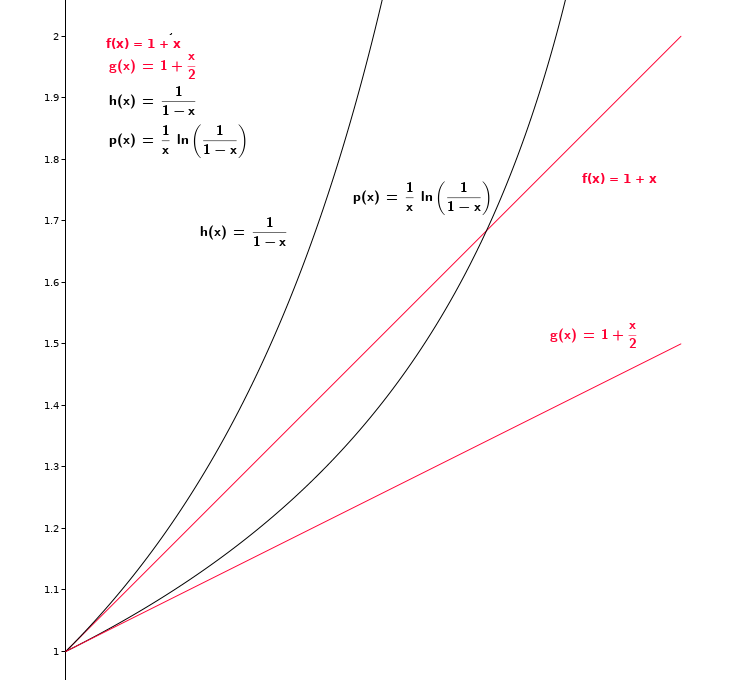
\includegraphics{images/image541.png}}

{Notiamo che i costi del concatenamento in nero (indirizzamento aperto) crescono molto più velocemente delle altre due rosse (liste di collisione).}
